\chapter{Úvod}
Tato práce se zabývá modely víceúrovňové autentizace. Jejím cílem je nalézt způsob pro přístup k jednomu zdroji z více univerzit za využití tamních přihlašovacích údajů.\\
Tato práce je součástí rozsáhlejší projektu Digitální kampus v rámci uskupení EULiST.
\\
Obsahuje základní informace o různých řešeních a dále se blíže zabývá modelem SSO v podobně standardu SAML a jeho konkrétní implementací Shibboleth.\\
Tato práce také obsahuje návody, jak zprovoznit Shibboleth SP, napojit ho na různé poskytovatele identity, což je ukázáno na Azure a SAMLtest, nastavení EDS pro využívání více IDP současně. A také využití Shibboleth SP s Apache2.\\
\\%IP2
V navazující IP2, bylo prozkoumáno několik CMS, a jejich možnosti SSO. K těmto prozkoumaným technologiím byly opět sepsány návody. Byla prozkoumána také další implementace SAML protokolu a to SimpleSamlPHP, včetně sepsání návodu k instalaci, nastavení a porovnání s technologií Shibboleth.



\section{Terminologie}
\subsection{Autentizace}
Proces ověření identity subjektu. Většinou následuje autorizace.\cite{Authorization}
\subsection{Autorizace}
Proces pro specifikování přístupových práv ke zdrojům.\cite{Autentizace}
 \subsection{Federované identity}
Způsob propojení identity uživatele napříč více nezávislými systémy. \cite{federatedIdentities}
\subsection{CMS} %IP2
Systém pro správu obsahu (CMS --- Content Management System) je software zajišťující správu dokumentů, nejčastěji webového obsahu.\cite{cms}

\chapter{Modely víceúrovňové autentizace}
\section{SSO}
\label{sso}
SSO (Single Sign-On) je mechanizmus pro jednotné přihlášení. Umožňuje uživateli se přihlásit na jednom místě a následně využívat toto přihlášení pro přístup k více nezávislým aplikacím. \cite{SSO}

\section{Proxy autentizace}
Je mechanizmus udržení identity a práv uživatele skrze více úrovní. Znamená to, že uživatel přistupuje celou dobu skrze aplikaci, na které se přihlásil, namísto přeposílání atributů třetí straně. Přihlašovací aplikace slouží tedy jako proxy server pro aplikaci třetí strany. \cite{ProxyA} \\ \\
Pro účely této práce není příliš vhodná, jelikož většina implementací nemá možnost předávání atributů, nebo jiný způsob odlišení jednotlivých uživatelů od sebe.

\subsection{EZproxy}
Jedná se o proxy server používaný převážně knihovnami, pro udělování přístupu, k jejich zdrojům uživatelům v různých sítích. Autentizace probíhá převážně pomocí IP adresy.\\
EZproxy nemá žádný mechanizmus pro odlišování různých uživatelů. Používá se tedy například pro přístup ke zdrojům knihovny pro celé univerzity. \cite{EZproxy}\cite{wikiEZproxy}

\chapter{SSO}

Nejvhodnější model víceúrovňové autentizace pro tuto práci je SSO, jelikož se zabývá federovanými identitami a spousta univerzit již využívá nějakou implementaci SSO.
Dále je uvedeno několik jeho implementací pomocí různých standardů. 

\section{SAML}

SAML\cite{SAMLofficialSite}\cite{WhatIsSaml} (Security Assertion Markup Language) je otevřený standard umožňující výměnu autentizačních a autorizačních dat mezi více nezávislými subjekty. Využívá k tomu protokol XML. 

SAML definuje tři role. Uživatel, poskytovatel identity (zkráceně IDP) a poskytovatel služeb (zkráceně SP). 

IDP se stará o autentizaci uživatele a následné poskytnutí dat SP.

SP se stará o autorizaci uživatele ke svým zdrojům na základě informací poskytnutých od IDP.


\subsection{Poskytovatel identity}

Poskytovatel identity se stará o autentizaci uživatelů. Poskytovatel identity po autentizaci uživatele předá poskytovateli služeb informaci o úspěšné autentizaci společně s různými atributy (například: e-mal, uživatelské jméno, role atd...).

\subsection{Poskytovatel služeb}

Poskytovatel služeb se stará o autorizaci přístupu k různým službám, které poskytuje na základě informací získaných od poskytovatele identity.

\subsection{Postup přihlášení za pomocí IDP}\label{IDPlogin}

Rozlišují se dvě možnosti přihlášení. Přihlášení vyvolané na straně IDP (obr. \ref{saml-flow-idp}) a přihlášení vyvolané na straně SP (obr. \ref{saml-flow-sp}).


Pokud bylo přihlášení vyvolané na straně SP, tak je uživatel přesměrován na IDP, kde bude vyzván k autentizaci.
Po úspěšné autentizaci IDP předá informaci o úspěšné autentizaci s různými uvolněnými atributy SP společně s přesměrováním uživatele na původní stránku.
Tyto informace SP využije k autorizaci různých svých částí uživateli.\cite{SAMLxOIDC}
\begin{figure}[!thbp]
	\centering
    \includegraphics[width=1\textwidth]{obrazky-figures/saml-sp-cropped.png}
	\caption{Ukázka přihlášení vyvolané SP\cite{SAMLxOIDC}}
	\label{saml-flow-sp}
\end{figure}

Pokud bylo přihlášení vyvolané na straně IDP, tak je uživatel rovnou přesměrován na SP s informací o úspěšné autentizaci společně s různými uvolněnými atributy.
Tyto informace SP využije k autorizaci různých svých částí.\cite{SAMLxOIDC}

\begin{figure}[!thbp]
	\centering
    \includegraphics[width=1\textwidth]{obrazky-figures/saml-idp-cropped.png}
	\caption{Ukázka přihlášení vyvolané IDP\cite{SAMLxOIDC}}
	\label{saml-flow-idp}
\end{figure}

\section{OIDC}

OIDC (OpenID Connect) je otevřený standard umožňující výměnu autentizačních a autorizačních dat mezi více nezávislými subjekty. Je postavený nad protokolem OAuth 2.0.\cite{OIDC}

\section{OAuth 2.0.}
Na rozdíl od OIDC OAuth 2.0. se stará pouze o autorizaci. Používá se většinou pro sdílení části dat uživatele s aplikací třetí strany bez předávání jeho přihlašovacích údajů. \\
OIDC je potom jeho nadstavba určená přímo pro federované identity. \cite{OAUTHvSAMLvOIDC}

\section{SAML versus OIDC}

SAML je starší z těchto dvou protokolů a využívá k přenosu dat XML. OIDC je novější a využívá k přenosu dat JSON. 
SAML je momentálně rozšířenější, i když OIDC nabírá na popularitě díky jednodušší implementaci a komunikaci přes JSON.\cite{SAMLxOIDC} \\
Princip přihlašování je až na různé názvosloví podobný (Service Provider (SP) = Relying Party (RP),  Identity Provider (IDP) = OpenID Provider (OP), atd ..).
Princip přihlašování je blíže popsán v sekci \ref{IDPlogin}.




\section{Shibboleth}

Shibboleth je implementace SAML standardu. Jeho hlavní součástí jsou dvě aplikace. Identity Provider (IDP), který slouží jako poskytovatel identity a stará se o autentizaci a Service Provider (SP), který slouží jako poskytovatel služeb a stará se o autorizaci po úspěšném přihlášení přes poskytovatele identity. \cite{shibbolethWiki}



\section{SimpleSamlPHP} %IP2

Jedná se o aplikaci napsanou v PHP, která se stará o autentizaci a autorizaci pomocí SAML protokolu. Jedná se o jednu z nejrozšířenějších opensource implementací SAML protokolu. Má jednoduché používání, dobrou dokumentaci a i spoustu pokročilejších funkcí.\cite{simplesamlphpdoc}
\\
Na rozdíl od Shibbolethu obsahuje IDP, SP a Discovery service v jedné aplikaci.

\section{SimpleSamlPHP výhody oproti Shibbolethu} %IP2

SimpleSamlPHP má přímočařejší a obsáhlejší dokumentaci, která pokrývá více jeho součástí, zatímco Shibboleth má spoustu nezdokumentovaných částí a hůře se v ní orientuje. SimpleSamlPHP je také rozšířenější a tedy existuje i více informací na internetu. Jeho nastavení je jednodušší, podporuje více IDP a SP na stejné instanci. Je možné nastavit specifické nastavení (např: mapování atributů) přímo pro jednotlivá IDP.\\ 
Spoustu věcí, které Shibboleth dělá odděleně, nebo má nejasně či složitě zdokumentované, obsahuje SimpleSamlPHP v jednom jednoduše nastavitelném balíčku (například discovery service je funkční ihned po instalaci SimpleSamlPHP). 

\chapter{Organizace a projekty} %IP2

Zde jsou organizace a projekty, do kterých je již velká část univerzit zapojená, které se starají o autentizaci a dají se tedy využít v rámci této práce.

\section{EULiST} %IP2
Jedná se o evropský projekt, v rámci kterého spolupracuje několik univerzit napříč Evropou a tvoří tak univerzitní alianci. Do této aliance v době psaní této práce patří Slovenská technická univerzita v Bratislave, Vysoké učení tehchnické v Brně,  Leibniz Universität Hannover, LUT University, Jönköping University, Rey Juan Carlos University, Technische Universität Wien, University of L’Aquila a Institut Mines-Télécom.\cite{eulist}
\\
Pro tuto organizaci vznikl projekt Digitální kampus, pro něhož je třeba zřídit přihlašování pomocí SSO, kterým se zabývá tato práce.

\subsection{Digitální kampus}

Jedná se o budoucí digitální infrastrukturu v rámci projektu EULiST pro vzdělání a výzkum, který bude mít za cíl usnadnit spolupráci mezi administrativními a akademickými pracovníky, studenty a širší komunitou EULiST.\cite{digitalcampus}

\section{EduGAIN} %IP2

EduGAIN je služba co se stará o propojení již existujících federací poskytovatelů identity. Toto velmi ulehčí přidávání a odebírání nových poskytovatelů identity a služeb, jelikož není pak třeba vyměnit si metadata s každým poskytovatelem identity/služeb. \\Do EduGAIN se mohou přidat pouze celé \emph{federace}. \cite{edugainWikipedie}\cite{edugain}\\
EduGAIN je převážně zaměřený na výzkum a vzdělání.
Do této služby je již velká část univerzit z projektu EULiST zapojena.

\section{EduID} %IP2

Jedná se o českou akademickou federaci identit, kterou zpravuje CESNET. 
Využívá ke své funkčnosti jako backend Shibboleth, ale je kompatibilní s jakoukoli SAML implementací, včetně SimpleSamlPHP. Členem Shibbolethu je i CESNET.\cite{eduid}
\\
Této federace využívá VUT, pro přístup do EduGAIN.

\chapter{Návody}
\label{návod}

V této kapitole jsou k nalezení návody na nastavení různých řešení pro zprovoznění SSO.

\section{Instalace Shibboleth SP} \label{instalaceShibboleth}

Zde následuje návod jak nainstalovat a nastavit Shibboleth SP tak, aby ho bylo možné propojit s IDP. Jedná se převážně o aktualizaci tohoto návodu\cite{shibbolethSpInstallation} v kombinaci s informacemi na oficiální wiki implementace Shibboleth\cite{shibbolethWikiSP}

Nejdříve je třeba nainstalovat web server. Tento návod využívá Apache2.
\begin{lstlisting}[language=Bash]
    sudo apt-get update
    sudo apt-get install apache2
\end{lstlisting}

Dále je třeba vygenerovat certifikáty pro Apache2. Pro jednoduchost se vygenerují self-signed certifikáty.
\begin{lstlisting}[language=Bash]
    sudo a2enmod ssl
    sudo a2ensite default-ssl.conf
    sudo mkdir /etc/apache2/ssl
    sudo openssl req -x509 -nodes -days 365 -newkey rsa:2048 \
    -keyout /etc/apache2/ssl/apache.key -out /etc/apache2/ssl/apache.crt
\end{lstlisting}

Shibboleth potřebuje vygenerovat certifikát ke komunikaci s IDP. Localhost je třeba nahradit IP adresou serveru, na kterém SP poběží.
\begin{lstlisting}[language=Bash]
    sudo shib-keygen -h localhost
    openssl x509 -text -noout -in /etc/shibboleth/sp-cert.pem
\end{lstlisting}

Nastavení Shibboleth se nachází v /etc/shibboleth/shibboleth2.xml .

\begin{lstlisting}[language=Bash]
   sudo vim /etc/shibboleth/shibboleth2.xml
\end{lstlisting}

Zde je potřeba nastavit následující hodnoty. \\V <ApplicationDefaults> je potřeba nastavit EntityID. EntityID by mělo být jedinečné v rámci federace. Většinou se používá doména aplikace, ke které se bude přistupovat přes Shibboleth s cestou /shibboleth. Například: http://vasedomena/shibboleth. Není to ale nutné pro fungování aplikace.

Pro povolení SSL je třeba nastavit v <Sessions>  handlerSSL na true a cookieProps na https.

Pod <SSO> se přidá EntityID IDP, který se bude používat.

Na konec souboru se přidá informace, kde se nachází metadata IDP.
\begin{lstlisting}[language=Bash]
 <MetadataProvider type="XML" validate="true"
                url="https://samltest.id/saml/idp"/>
\end{lstlisting}

Pro jednoduchost se použije jeden klíč pro podpis i pro šifrování.

Toho se docílí změnou těchto řádků:
\begin{lstlisting}[language=Bash]
<CredentialResolver type="File" use="signing"
            key="sp-signing-key.pem" certificate="sp-cert.pem"/>
<CredentialResolver type="File" use="encryption"
            key="sp-encrypt-key.pem" certificate="sp-cert.pem"/>
\end{lstlisting}

Na následující:
\begin{lstlisting}[language=Bash]
<CredentialResolver type="File"
            key="sp-key.pem" certificate="sp-cert.pem"/>
\end{lstlisting}

Dále je třeba restartovat Shibboleth.
\begin{lstlisting}[language=Bash]
sudo service shibd restart
\end{lstlisting}

Pokud je vše nastaveno správně, tak na následující adrese bude text: "A valid session was not found."\\
\url{https://vasedomena/Shibboleth.sso/Session}

\section{Propojení Shibboleth s IDP}

Zde je uvedeno pár návodů pro propojení SP s různými IDP.

\subsection{SAMLtest}
SAMLtest je testovací stránka pro debugování SAML aplikací. Většina IDP bude mít stejný postup propojení jako SAMLtest.



Na následující adresu je třeba nahrát metadata z SP 
\url{https://samltest.id/upload.php}. Ty se dají získat na následující cestě na doméně, kde je hostován SP \url{https://vasedomena//Shibboleth.sso/Metadata}.

Dále je potřeba v nastavení Shibboleth SP (/etc/shibboleth/shibboleth2.xml) přidat cestu k metadatům IDP.
\begin{lstlisting}[language=Bash]
 <MetadataProvider type="XML"
                url="https://samltest.id/saml/idp"/>
\end{lstlisting}

Teď, když se zajde na stránku \url{https://samltest.id/start-sp-test/}, tak po vyplnění entityID se dá přihlásit do SP přes SAMLtest IDP.

Po přihlášení by měly být vidět na následující adrese informace o aktivní relaci \url{http://vasedomena/Shibboleth.sso/Session}.

\subsection{VUT}
Propojení s poskytovatelem identity VUT je velice podobné jako propojení se SAMLtest.



Je třeba VUT zaslat metadata SP. Ty se dají získat na následující cestě na doméně, kde je hostován SP \url{https://vasedomena//Shibboleth.sso/Metadata}.

Dále je potřeba v nastavení Shibboleth SP (/etc/shibboleth/shibboleth2.xml) přidat cestu k metadatům IDP.
\begin{lstlisting}[language=XML]
 <MetadataProvider type="XML"
  url="https://app.fit.vut.cz/simplesaml/saml2/idp/metadata.php"/>
\end{lstlisting}

Změna oproti SAMLtest je že IDP od VUT nepodepisuje logout odpovědi, takže je třeba nastavit u SP ignorování nepodepsaných logout odpovědí. To se udělá následovně.\\
V souboru  "/etc/shibboleth/security-policy.xml" přidat následující řádky:
\begin{lstlisting}[language=XML]
<!-- Turns off the requirement of having signed LogoutResponses -->
<Policy id="unsigned-slo">
  <PolicyRule type="NullSecurity"/>
</Policy>
\end{lstlisting}

 v nastavení Shibboleth SP (/etc/shibboleth/shibboleth2.xml)
 změnit tento řádek:
 \begin{lstlisting}[language=XML]
 <Logout>SAML2 Local</Logout>
\end{lstlisting}
na tento:
 \begin{lstlisting}[language=XML]
 <Logout conf:policyId="unsigned-slo">SAML2 Local</Logout>
\end{lstlisting}

Teď, když se zajde na stránku \url{https://samltest.id/start-sp-test/}, tak po vyplnění entityID se dá přihlásit do SP přes SAMLtest IDP.

Po přihlášení by měly být vidět na následující adrese informace o aktivní relaci \url{http://vasedomena/Shibboleth.sso/Session}.

\subsection{Azure}

Tato sekce je inspirována tímto návodem.\cite{AzureTutorial}
\\
\\
Pro propojení s Azure IDP je potřeba udělat následující kroky:
\begin{itemize}
    \item nejprve je potřeba vytvořit aplikaci, která bude sloužit jako IDP
    \begin{itemize}
    \item v Azure Portalu u Azure Services je třeba kliknout na Azure Active Directory
    \item vlevo ve sloupci pod manage otevřít Enterprise applications
    \item kliknout na New application
    \item kliknout na Create your own application
    \item tlačítkem Create potvrdit vytvoření aplikace
    \end{itemize}
    \item v aplikaci vlevo pod položkou Single sign-on se vybere SAML a dále je potřeba nastavit následující
    \item Basic SAML Configuration
    \begin{itemize}
        \item Identifier je třeba nastavit na entityID SP
        \item Reply URL je třeba nastavit na \url{https://vasedomena/Shibboleth.sso/SAML2/POST}
    \end{itemize}
    \item \mbox{Attributes \& Claims} \linebreak
    Protože Azure využívá pro NameID SAML identifier místo SAML atributu, tak je potřeba pro NameID nastavit Name identifier format na Unspecified.
    Dále stačí vybrat, jaký atribut se bude používat pro identifikaci uživatele.
    
    Poté je ještě potřeba v nastavení SP v souboru attribute-map.xml (/etc/shibboleth/attribute-map.xml) přidat následující řádky:
    
\begin{lstlisting}[language=XML]
   <Attribute name="urn:oasis:names:tc:SAML:1.1:nameid-format:unspecified"
   id="NameID">
        <AttributeDecoder xsi:type="NameIDAttributeDecoder" 
        formatter="$Name" defaultQualifiers="true"/>
   </Attribute>
\end{lstlisting}
které řeknou Shibboleth jak interpretovat NameID. NameID bude uloženo v proměnné NameID.

Jakékoli další atributy, které je potřeba předávat SP, se dají nastavit na této stránce podobným způsobem. Name format se nechá na Omitted, jinak zbytek nastavení je dle potřeb aplikace. Následně je potřeba do attribute-map.xml přidat informaci, jak se mají jednotlivé atributy zpracovat.
   \begin{lstlisting}[language=XML]
     <Attribute name="Namespace/Name"
    nameFormat="urn:oasis:names:tc:SAML:2.0:attrname-format:unspecified"
    id="role1" />
    \end{lstlisting}
Namespace se nahradí za namespace atributu. Name se nahradí za název atributu a do id se nastaví název proměnné, do které se má atribut namapovat. Pokud bylo potřeba měnit Name Format, tak je ho potřeba změnit i zde.\cite{AddAttribute}
    


    \item Dále je třeba nahrát pomocí tlačítka vlevo nahoře "Upload metadata file" metadata SP. Tato metadata jsou k nalezení na této cestě u vašeho SP \url{http://vasedomena/Shibboleth.sso/Metadata}.

\end{itemize}

Po nastavení se dá aplikace otestovat tlačítkem Test. Aplikace by vás měla přesměrovat na doménu vaší aplikace a následně na následující adrese \url{https://vasedomena/Shibboleth.sso/Session} by měla být vidět aktivní relace a názvy atributů, které IDP předal SP.

\section{Používání v Apache}

Pro využití Shibboleth v Apache stačí uvést do .htaccess, co je vyžadováno za oprávnění od uživatele. Více informací o syntaxi je k nalezení v dokumentaci\cite{SPApache}\cite{SPhtaccess}. \linebreak

Příklad .htaccess pro přístup uživatele testuser@gmail.com:

 \begin{lstlisting}[language=xml]
    # nastavi typ prihlasovani na Shibboleth
    AuthType shibboleth
    # nastavi vyzadovani Shibboleth session
    ShibRequestSetting requireSession true
    # nasledujici blok nastavi, ze je vyzadovana kombinace techto parametru
<RequireAll>
  # nastavi, ze je vyzadovan shibboleth k pristupu
  require shibboleth 
  # nastavi pristup pro uzivatele s id testuser@gmail.com
  require shib-user testuser@gmail.com 
</RequireAll>
    \end{lstlisting}


\section{Shibboleth discovery service}
Pro používání více než jednoho IDP je potřeba nastavit discovery service, kde si může uživatel vybrat jakého poskytovatele identity chce použít. Pro jednoduché řešení stačí statická webová stránka s přesměrováními na různé poskytovatele služeb, pro řešení obsahující více IDP je lepší využít discovery service od Shibboleth. Různé možnosti implementace jsou popsané v dokumentaci \cite{IdPDiscovery}.

\subsection{Embedded Discovery Service}
Je jednoduchá discovery service od Shibboleth napsaná v javascriptu. 

\subsection{Embedded Discovery Service - návod}
Tato sekce byla inspirována následujícím návodem \cite{EDS-tut}. \\ \\
instalace EDS:
\begin{lstlisting}[language=Bash]
sudo su -

cd /usr/local/src

wget https://shibboleth.net/downloads/embedded-discovery-service/\
latest/shibboleth-embedded-ds-1.2.2.tar.gz -O shibboleth-eds.tar.gz

tar xzf shibboleth-eds.tar.gz

cd shibboleth-embedded-ds-1.2.2

apt install make

make install
\end{lstlisting}

povolení webové stránky EDS

\begin{lstlisting}[language=Bash]
mv /etc/shibboleth-ds/shibboleth-ds.conf \
/etc/apache2/conf-available/shibboleth-ds.conf

a2enconf shibboleth-ds.conf

systemctl restart apache2.service
\end{lstlisting}

V Shibboleth SP nastavení (/etc/shibboleth/shibboleth2.xml) je třeba upravit následující:\\
 \begin{itemize}
    \item
SSO změnit následovně:

\begin{lstlisting}[language=Bash]
<SSO discoveryProtocol="SAMLDS" 
     discoveryURL="https://vasedomena/shibboleth-ds/index.html">
   SAML2 SAML1
</SSO>
\end{lstlisting}
\item
odkomentovat DiscoveryFeed handler a SessionInitiator handler

\begin{lstlisting}[language=xml]
<Handler type="DiscoveryFeed" Location="/DiscoFeed"/>
<Handler type="SessionInitiator" Location="/Login"/>
\end{lstlisting}
\end{itemize}
Následně je třeba restartovat Shibboleth SP a Apache2.

\begin{lstlisting}[language=Bash]
systemctl restart shibd.service
systemctl restart apache2.service
\end{lstlisting}

Dále je potřeba nastavit whitelist návratových adres v souboru idpselect\_config.js, který se nachází v nastavení EDS (/etc/shibboleth-ds/idpselect\_config.js).

V položce this.returnWhiteList je třeba změnit url aby odpovídala vašemu SP. 

\begin{lstlisting}[]
this.returnWhiteList = 
["^https:\/\/vasedomena\.com\/Shibboleth\.sso\/Login.*$",
 "^https:\/\/vasedomena\.com\/Shibboleth\.sso\/Login.*$"];
\end{lstlisting}

Teď, když se zkusí zajít na nějaký zdroj chráněný pomocí Shibboleth, tak dojde k přesměrování na stránku podobné té na obrázku \ref{EDS}.

\begin{figure}[hbp]
	\centering
    \includegraphics[width=0.6\textwidth]{obrazky-figures/disc.png}
	\caption{Ukázka EDS}
	\label{EDS}
\end{figure}

Zde si může uživatel jednoduše vybrat IDP, na jehož přihlašovací stránku chce být přesměrován.

\section{SimpleSamlPHP} %IP2
V této sekci jsou veškeré návody potřebné k základnímu nastavení SimpleSamlPHP.
\subsection{Instalace}
Návod na instalaci SimpleSamlPHP je k nalezení na následujících webových stránkách \cite{SimpleSAMLphp-instalation-and-configurationduid}. Jedná se o oficiální dokumentaci SimpleSAMLphp. Tento návod byl v rámci této práce otestován, a nebylo potřeba ho nějak aktualizovat.

\subsection{Nastavení} %IP2
K základnímu nastavení slouží soubor config.php, který se nachází v adresáři simplesamlphp/config.

K nastavení metadat slouží soubory ve složce simplesamlphp/config/metadata. Zde se nachází soubory pro nastavení metadat pro IDP, které SP využívá, pro SAML IDP se využívá soubor saml20-idp-remote.php.

Mapování atributů lze nastavit na více místech, více v sekci \ref{attributemap_ssphp}.

Pro nastavení kromě config souborů existuje i administrační stránka, která je dostupná na adrese vase.domena/simplesaml. Zde je možné nastavit některé parametry, které jsou v config souborech, ale většinu nastavení je potřeba upravovat přes config soubory.
Více informací v dokumentaci. \cite{simplesamlphpdoc}

\subsubsection{Přidávání nových IDP} %IP2

Pro přidání IDP stačí do souboru simplesamlphp/config/metadata/saml20-idp-remote.php přidat nový záznam.

Získat metadata ve správném formátu lze pomocí aplikace na stránce nastavení vaší instance SimpleSamlPHP vase.domena/simplesaml.
Zde po přihlášení v záložce \emph{federation}, je nástroj \emph{XML to SimpleSamlPHP metadata converter}, který po nahrání metadat převede metadata do správného formátu.
Více informací je k nalezení v dokumentaci.\cite{SimpleSAMLphp-Service-Provider-QuickStart}
\\
Zde následuje příklad metadat pro vutbr.cz (některé informace byli z důvodu bezpečnosti odstraněny).
\begin{lstlisting}

    $metadata['https://app.fit.vut.cz/simplesaml/saml2/idp/'] = array (
        'entityid' => 'https://app.fit.vut.cz/simplesaml/saml2/idp/',
        'description' =>
        array (
          'en' => 'Faculty of information technology BUT',
          'cs' => 'Fakulta informačních technologií VUT',
        ),
        'OrganizationName' =>
        array (
          'en' => 'Faculty of information technology BUT',
          'cs' => 'Fakulta informačních technologií VUT',
        ),
        'name' =>
        array (
          'en' => 'Faculty of information technology BUT',
          'cs' => 'Fakulta informačních technologií VUT',
        ),
        'OrganizationDisplayName' =>
        array (
          'en' => 'Faculty of information technology BUT',
          'cs' => 'Fakulta informačních technologií VUT',
        ),
        'url' =>
        array (
          'en' => 'https://www.fit.vut.cz/.en',
          'cs' => 'https://www.fit.vut.cz/.cs',
        ),
        'OrganizationURL' =>
        array (
          'en' => 'https://www.fit.vut.cz/.en',
          'cs' => 'https://www.fit.vut.cz/.cs',
        ),
        'contacts' =>
        array (
          0 =>
          array (
            'contactType' => 'support',
            'company' => 'CVT FIT VUT',
            'givenName' => 'Jmeno',
            'surName' => 'Prijmeni',
            'emailAddress' =>
            array (
              0 => 'mail',
            ),
            'telephoneNumber' =>
            array (
              0 => '123 123 123',
            ),
          ),
          1 =>
          array (
            'contactType' => 'technical',
            'givenName' => 'jmeno',
            'emailAddress' =>
            array (
              0 => 'mailto:mail',
            ),
          ),
        ),
        'metadata-set' => 'saml20-idp-remote',
        'sign.authnrequest' => true,
        'SingleSignOnService' =>
        array (
          0 =>
          array (
            'Binding' => 'urn:oasis:names:tc:SAML:2.0:bindings:HTTP-Redirect',
            'Location' => 'https://app.fit.vut.cz/simplesaml
            /saml2/idp/SSOService.php',
          ),
        ),
        'SingleLogoutService' =>
        array (
          0 =>
          array (
            'Binding' => 'urn:oasis:names:tc:SAML:2.0:bindings:HTTP-Redirect',
            'Location' => 'https://app.fit.vut.cz/simplesaml
            /saml2/idp/SingleLogoutService.php',
          ),
        ),
        'ArtifactResolutionService' =>
        array (
        ),
        'NameIDFormats' =>
        array (
          0 => 'urn:oasis:names:tc:SAML:2.0:nameid-format:transient',
        ),
        'keys' =>
        array (
          0 =>
          array (
            'encryption' => false,
            'signing' => true,
            'type' => 'X509Certificate',
            'X509Certificate' => 'zde by byl certifikát',
          ),
          1 =>
          array (
            'encryption' => true,
            'signing' => false,
            'type' => 'X509Certificate',
            'X509Certificate' => 'zde by byl certifikát',
          ),
        ),
      );

\end{lstlisting}

\subsubsection{Mapování a filtrování atributů}\label{attributemap_ssphp} %IP2
Mapování atributů lze nastavit na různých místech dle potřeby.

\begin{itemize}

    \item Globálně v config.php.
    \item Specificky pro jednotlivé SP v authsources.php.
    \item Specificky pro jednoho IDP v saml20-idp-remote.

\end{itemize}

Jedno ze základních jednoduchých mapování je například přejmenování atributu. Toto se dělá pomocí \emph{core:AttributeMap}.

\begin{lstlisting}[json]
    'authproc' => [
        50 => [
            'class' => 'core:AttributeMap',
            'urn:oasis:names:tc:SAML:attribute:subject-id' => 'subject-id',
            'urn:oid:2.5.4.20' => 'phone',
        ],
    ],
\end{lstlisting}

Toto nastavení namapuje \emph{urn:oasis:names:tc:SAML:attribute:subject-id} na \emph{subject-id} a \emph{urn:oid:2.4.20} na \emph{phone}. Nastavení se dá dělat globálně, specificky pro SP nebo specificky pro IDP.

Další možnosti filtrování jsou například
\begin{itemize}
    \item core:AddAttributeAdd - přidá atribut
    \item core:AttributeAlter - vyhledá a nahradí hodnoty atributu
    \item core:AttributeNameId - vygeneruje NameID z hodnoty atributu
\end{itemize}

Mapování a filtrování atributů je dále podrobněji popsáno v dokumentaci SimpleSamlPHP. \cite{Authentication-Processing-Filters-in-SimpleSAMLphp}


\subsubsection{Nalezení názvů atributů} %IP2
Vyhledání názvů uvolněných atributů z IDP lze nalézt v administraci SimpleSamlPHP vase.domena/simplesaml v záložce \emph{Authentication} -> \emph{Test configured authentication sources} -> \emph{Vyberte vaseho SP} -> \emph{vyberte IDP od kterého chcete vyhledat uvolněné attributy}. Dále se po přihlášení v IDP zobrazí všechny atributy, které jsou uvolněny z IDP.


\section{Wordpress} %IP2

Wordpress je opensource CMS napsaný v PHP, který je zaměřený na jednoduchost používání a rozšířitelnost pomocí pluginů. Jedná se o jeden z nejrozšířenějších CMS. Více informací je k nalezení na webových stránkách\cite{wordpress}.
\\
Následují návody ke zprovoznění SSO ve Wordpressu.

\subsection{SSO plugin} %IP2
Do Wordpressu byl otestován jeden plugin na napojení Shibboleth SP k Wordpressu. Jedná se o plugin Shibboleth SP\cite{ShibbolethSpWp}. Tento plugin funguje, ale obsahuje jen základní nastavení a většinu věcí přenechává samotnému Shibbolethu.

\subsection{Instalace Shibboleth pluginu} %IP2
Plugin vyžaduje aby byl již nainstalován Shibboleth SP. K tomuto lze využít návod v této sekci \ref{instalaceShibboleth}. Dále je potřeba upravit \emph{.htaccess} Wordpressu, aby ignoroval url cesty \emph{/Shibboleth.sso}. Tohoto lze například docílit úpravou \emph{.htaccess} v kořenovém adresáři Wordpressu do následující podoby.

\begin{lstlisting}[language=php]

<IfModule mod_rewrite.c>
RewriteEngine On
RewriteRule .* - [E=HTTP_AUTHORIZATION:%{HTTP:Authorization}]
RewriteBase /
RewriteRule ^index\.php$ - [L]
RewriteCond %{REQUEST_URI} !^/Shibboleth.sso/.*$
RewriteCond %{REQUEST_FILENAME} !-f
RewriteCond %{REQUEST_FILENAME} !-d
RewriteRule . /index.php [L]
</IfModule>


\end{lstlisting}

Po té stačí nainstalovat plugin a nastavit mu následující parametry.

\begin{enumerate}
    \item V záložce \emph{general}
    \begin{enumerate}
        \item Nastavit \emph{login URL} na \emph{vase.domena/Shibboleth.sso/Login}.
        \item Nastavit \emph{logout URL} na \emph{vase.domena/Shibboleth.sso/Logout}.
    \end{enumerate}
    \item V záložce \emph{User}.
     \begin{enumerate}
        \item Nastavit mapování atributů na proměnné Wordpressu, zadávají se sem parametry namapované v \emph{attribute-map.xml}.
        \item Zaškrtnou přepínač \emph{Automaticly create users if they do not exist in Wordpress database} pro automatické vytvoření uživatele při prvním přihlášení přes idp.
     \end{enumerate}
\end{enumerate}

Toto je základní nastavení pro aktivování SSO.

\section{Drupal} %IP2

Drupal je také opensource CMS napsaný v PHP, který je zaměřený na rozšířitelnost pomocí pluginů (Drupal je nazývá moduly). Je to jeden z nejrozšířenějších CMS. Oproti Wordpressu má o trochu strmější učící křivku, jelikož je spíše zaměřen na vývojáře, zatímco Wordpress je více přátelský pro začátečníky a neprogramátory. \cite{drupalvswordpress} 
Více informací lze nalézt na webových stránkách.\cite{drupal}
\\
Následují návody ke zprovoznění SSO v Drupalu.

\subsection{SSO plugin} %IP2
Drtivá většina modulů na SSO pro Drupal využívá nějaký již nainstalovaný backend na hostitelském serveru, většinou SimpleSamlPHP a některé také Shibboleth. Dále jsou zde i komerční moduly jako například od miniOrange\cite{miniorange}, které jsou většinou již hotová řešení, kde stačí nainstalovat modul. Z důvodu lepší modularity a rozšířitelnosti bylo vybráno opensource řešení v podobě SimpleSamlPHP.

\subsubsection{Shibboleth modul} %IP2
    Drupal nemá žádný dobrý Shibboleth modul, který by byl udržovaný, fungoval jednoduše hned po instalaci a měl by nějaké lepší funkce. Nejlepší modul co se povedlo nalézt je tento\cite{basicshib}. Bohužel se ale zdá že v současnosti není funkční.
\subsubsection{SimpleSamlPHP} %IP2
    Drupal má skvělý modul pro propojení se SimpleSamlPHP, který je velmi jednoduchý na používání a má i nějaké pokročilejší funkce. Jedná se o tento plugin \cite{SimpleSAMLphpDrupal}.
\\ 
\\
     Podporované funkce v době psaní této práce (převzato z \cite{SimpleSAMLphpDrupal}):
    \begin{itemize}
        \item Instantní vytváření uživatelských účtů na základě SAML atributů (konfigurovatelné).
        \item Automatické přiřazování rolí na základě SAML atributů (konfigurovatelné).
        \item Duální mód - podpora tradičních Drupal účtů a SAML-autentizovaných účtů současně (konfigurovatelné).
        \item  Podpora více autentizačních protokolů (díky SimpleSamlPHP)
        \begin{itemize}
            \item OpenID (např. Google, Yahoo)
            \item Facebook
            \item OAuth (např. Twitter)
            \item SAML 1.1, SAML 2.0
            \item Shibboleth 1.3
            \item A-Select
            \item X509 Client Certificates
            \item Radius
        \end{itemize}
    \end{itemize}
    \\
    Příklady použití (převzato z \cite{SimpleSAMLphpDrupal}):
    \begin{itemize}
        \item Enterprise single sign-on --- připojte Drupal stránky k IDP vaší organizace (stejně jako připojení Google Apps k vašemu IdP)
        \item Single sign-on napříč Drupal stránkami na více serverech --- nastavte všechny stránky tak, aby používaly tento modul k ověřování uživatelů proti jednomu nebo více IDP. (To lze dokonce provést s více stránkami, které používají jediného poskytovatele služeb SimpleSamlPHP.)
        \item Federovaná Drupal stránka --- umožněte lidem z více organizací přistupovat na stránku pomocí IdP jejich organizace.
        \item Přihlášení pomocí Facebooku/Googlu/Twitteru/atd... --- umožněte uživatelům přihlásit se na vaši stránku pomocí jejich účtu na některé z těchto služeb.
    \end{itemize}
    
\subsubsection{Instalace SimpleSamlPHP modulu} %IP2

Modul se instaluje jako každý jiný Drupal modul. Modul je k nalezení zde \cite{SimpleSAMLphpDrupal}.

SimpleSamlPHP je potřeba mít nastavené aby používalo něco jiného než \emph{phpsession} jako úložiště relace. Jako úložiště relace se dá použít \emph{memcache} nebo \emph{SQL}.
Toto lze nastavit v \emph{simplesamlphp/config/config.php} v proměnné \emph{store.type}.
Nejjednodušší je nastavit memcache. Další informace lze nalézt na stránkách modulu \cite{SimpleSAMLphpDrupal}.

\subsubsection{Nastavení SimpleSamlPHP modulu} %IP2

Pro základní spuštění stačí v nastavení modulu v Drupalu nastavit následující:

\begin{enumerate}
    \item V \emph{User info and syncing} nastavit atributy které se mají namapovat na atributy Drupalu.
    \item V \emph{Basic settings}:
    \begin{enumerate}
        \item Nastavit \emph{Authentication source for this SP} na vašeho sp.
        \item Po dokončení nastavení můžete modul aktivovat pomocí \emph{Activate authentication via SimpleSamlPHP}.
    \end{enumerate}

\end{enumerate}

\chapter{Plán pluginu}

Zde jsou možnosti co by se dalo rozšířit na SimpleSamlPHP při integraci do digitálního kampusu.

\section{možná rozšíření}

\begin{itemize}
    \item Přidat možnost přidávat/editovat/odebírat IDP přes gui (buď v Drupal modulu nebo v SimpleSamlPHP administraci).
    \item Automatické plnění jakýchkoli Drupal atributů.
    \item Export/import kompletního nastavení jak modulu tak SimpleSamlPHP.
    \item Možnost deaktivovat aktualizaci atributů pro jednotlivé uživatele.
\end{itemize}

\subsection{Automatické plnění jakýchkoli Drupal atributů}
K tomuto lze využít například tento plugin, je funkční hned po instalaci. \cite{SimpleSAMLphpDrupalAttr}

\subsection{Přidávání/odebírání/deaktivace/nastavení IDP přes gui}
Možnost upravovat IDP přímo z modulu/administrace SimpleSamlPHP bez nutnosti editovat config soubory. 
Pomocí jednoduchého menu by bylo možné přidat IDP. Následně nastavit url/nahrát jeho metadata.
Zde by mohlo být i možné nastavit přemapování přijatých atributů od konkrétního IDP na standardizované atributy v rámci Drupalu.

\subsection{Mazání již neexistujících uživatelů }
Pro tuto funkcionalitu bude třeba otestovat jestli IDP daných univerzit podporují nějaký způsob dotázání se jestli daný uživatel existuje v jejich IDP, jelikož tuto vlastnost SAML nespecifikuje.\\

\subsection{Možnost deaktivovat aktualizaci atributů pro jednotlivé uživatele}
Mohou existovat výjimky, kde bude třeba nastavit data ručně, z tohoto důvodu se může hodit možnost deaktivovat automatické nahrávání atributů pro jednotlivé uživatele.

\section{Usecase diagram}

K samotnému pluginu bude mít přístup pouze administrátor/technický pracovník.

\\ \\

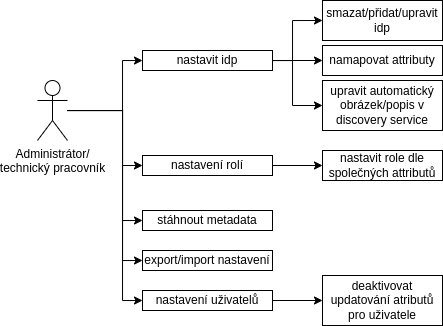
\includegraphics[scale=0.8]{obrazky-figures/usecase-diagram.png}



    



    % \chapter{Config Shibbolethu} 
    % Popis důležitých částí nastavení, které jsou nutné k správnému fungování Shibboleth SP. Detailní informace jsou k nalezení na webu\cite{SPconfig}. 
    
    % \section{shibboleth2.xml}
    % Hlavní config soubor Shibboleth SP. Nachází se na cestě /etc/shibboleth/shibboleth2.xml .
    
    % \subsection{ApplicationDefaults}
    % \begin{lstlisting}[language=xml]
    % <ApplicationDefaults entityID="https://vasedomena/shibboleth"
    %         REMOTE_USER="NameID"
    %         cipherSuites="DEFAULT:!EXP:!LOW:!aNULL:!eNULL:!DES:!IDEA:
    %         !SEED:!RC4:!3DES:!kRSA:!SSLv2:!SSLv3:!TLSv1:!TLSv1.1">
    % \end{lstlisting}
    % \begin{itemize}
    %     \item entityID \linebreak
    %     Název SP. Musí být unikátní v rámci federace identit. Je zvykem využít doménu SP s cestou /shibboleth.  
    %     \item REMOTE\_USER \linebreak
    %     Zde patří názvy atributů od různých IDP, které slouží k identifikaci uživatele. 
    %     Tento atribut bude následně k dispozici z proměnné REMOTE\_USER.
    % \end{itemize}
    % \subsection{MetadataProvider}
    % Definuje, kde se nachází metadata IDP. Pro většinu aplikací by mělo stačit jedno z následujících nastavení. Více informací lze nalézt na webových stránkách\cite{MetadataProvider}.
    % \linebreak \linebreak
    % Metadata se nahrávají z url.
    % \begin{lstlisting}[language=Bash]
    %  <MetadataProvider type="XML" validate="true"
    %                 url="https://samltest.id/saml/idp"/>
    % \end{lstlisting}
    % Metadata se nahrávají ze souboru.
    % \begin{lstlisting}[language=Bash]
    %  <MetadataProvider type="XML" path="/path/to/the/metadata.xml"/>
    % \end{lstlisting}
    
    
    % \section{attribute-map.xml}
    % Obsahuje informace o mapování atributů přijatých od IDP na proměnné SP. Soubor obsahuje nějaké základní mapování, ale pro většinu aplikací bude nutné tento soubor upravit.
    
    % Následuje příklad přidání jednoduchého atributu, kde jméno atributu přijatého od IDP je FavoriteFruit a favFruit je jméno používané v proměnných SP\cite{AddAttribute}.
    %  \begin{lstlisting}[language=XML]
    %      <Attribute name="FavoriteFruit"
    %     nameFormat="urn:oasis:names:tc:SAML:2.0:attrname-format:basic"
    %     id="favFruit" />
    %     \end{lstlisting}
        
    % Toto nastavení by mělo být dostačující pro většinu aplikací. Více informací lze nalézt na webových stránkách\cite{AddAttribute}.


\chapter{Závěr}


V úvodu bylo prozkoumáno několik různých modelů pro víceúrovňovou autentizaci. Z těchto modelů bylo pro potřeby projektu zvoleno SSO, jelikož umožňovalo federovat identity uživatelů mezi více institucí s technologiemi, které již byly na těchto institucích většinou implementovány a také pro jednoduchou rozšiřitelnost o další instituce.
\\
Z používaných technologií byl zvolen SAML, protože již existovala jeho implementace přímo pro potřeby univerzit a společně s OIDC patří k nejrozšířenějším SSO technologiím. \\
Touto implementací je Shibboleth, který je na řadě univerzit již implementován, nebo je implementován nějaký IDP, který je s ním kompatibilní (Azure, Google Suite, atd...).\\
Podařilo se nastavit Shibboleth SP pro základní přihlašování se dvěma poskytovateli identit (SAMLtest a Azure) a byly sepsány stručné návody pro základní zprovoznění SP, jeho napojení na 2 různé IDP, propojení s webovým serverem Apache2 a nastavení EDS pro využívání více IDP.

%IP2 
V navazující IP2 bylo prozkoumáno několik CMS, blíže byly otestovány dva Drupal a Wordpress a byli také otestovány možnosti SSO v těchto CMS. 
Jako hlavní CMS byl nakonec zvolen Drupal, jelikož s Wordpressem si je velice podobný, a zároveň jsem měl s ním více zkušeností. Pro Drupal byl vybrán modul SimpleSamlPHP, který je jednoduchý na používání a má už hotový kvalitní modul, na který bude jednoduché navázat. 
\\
SimpleSamlPHP bylo také zvoleno z důvodu, lepší dokumentace, více funkcí a většímu celkovému rozšíření.
\\
Taky byl přidán popis organizací EduGAIN a EduID, které budou v rámci navazujícího projektu využívány.


\label{zaver}






%===============================================================================